% A literal cap-closure decomposition; all tangle interiors are retained.
% Build with pdfLaTeX; the PDF supplies the SVG and PNG exports.
\documentclass[tikz,border=12pt]{standalone}
\usepackage[T1]{fontenc}
\usepackage{lmodern,amsmath}
\usetikzlibrary{arrows.meta,calc}
\definecolor{ink}{HTML}{183444}
\definecolor{blue}{HTML}{1B6780}
\definecolor{amber}{HTML}{AD601A}
\newcommand{\tanglebox}[3]{%
  \draw[draw=blue,fill=blue!5,rounded corners=2pt]
    (#1-.9,#2-.55) rectangle (#1+.9,#2+.55);
  \node[font=\Large] at (#1,#2) {$#3$};
  \foreach \dx in {-.45,.45}{
    \fill[ink] (#1+\dx,#2-.55) circle(1.6pt);
    \fill[ink] (#1+\dx,#2+.55) circle(1.6pt);
  }
}
\newcommand{\uppercap}[3]{%
  \draw[#3] (#1-.45,#2)--(#1-.45,#2+.25)
    .. controls (#1-.45,#2+.85) and (#1+.45,#2+.85) ..
    (#1+.45,#2+.25)--(#1+.45,#2);
}
\newcommand{\lowercap}[3]{%
  \draw[#3] (#1-.45,#2)--(#1-.45,#2-.25)
    .. controls (#1-.45,#2-.85) and (#1+.45,#2-.85) ..
    (#1+.45,#2-.25)--(#1+.45,#2);
}
\begin{document}
\hyphenpenalty=10000\exhyphenpenalty=10000
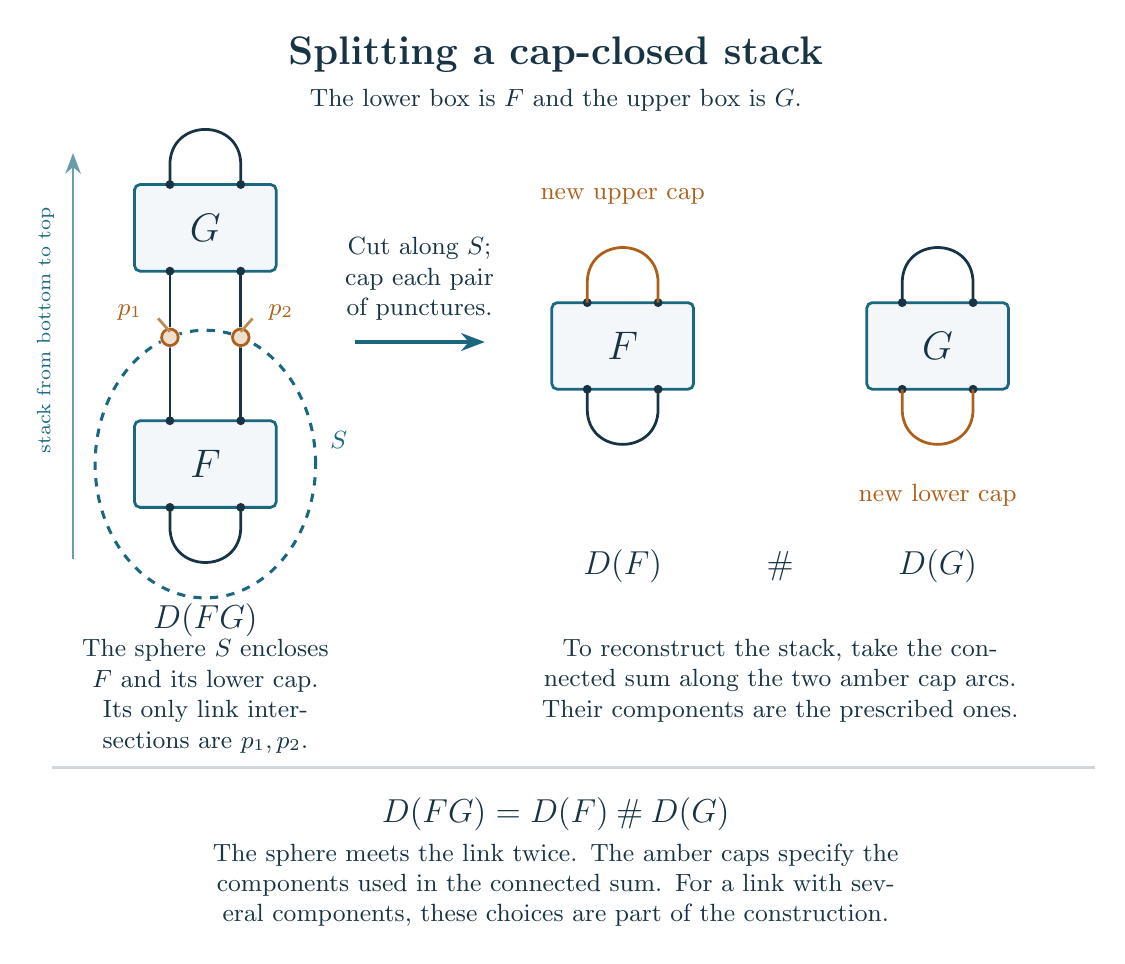
\begin{tikzpicture}[font=\sffamily,text=ink,line width=1pt,>=Stealth]
  \node[font=\Large\bfseries] at (6.25,3.7)
    {Splitting a cap-closed stack};
  \node[font=\small,align=center] at (6.25,3.12)
    {The lower box is $F$ and the upper box is $G$.};

  % The original cap closure, with two actual interface strands.
  \draw[blue,dashed,line width=1.1pt] (1.8,-1.5) ellipse(1.4 and 1.7);
  \tanglebox{1.8}{-1.5}{F}
  \tanglebox{1.8}{1.5}{G}
  \uppercap{1.8}{2.05}{ink}
  \lowercap{1.8}{-2.05}{ink}
  \foreach \dx in {-.45,.45}{
    \draw[ink] (1.8+\dx,-.95)--(1.8+\dx,.95);
  }
  \pgfmathsetmacro{\punctureheight}{-1.5+1.7*sqrt(1-(.45/1.4)^2)}
  \foreach \dx in {-.45,.45}{
    \fill[white] (1.8+\dx,\punctureheight) circle(3.7pt);
    \draw[amber,fill=amber!20] (1.8+\dx,\punctureheight) circle(3pt);
  }
  \node[font=\small,text=amber,anchor=east] at (1.13,.43) {$p_1$};
  \node[font=\small,text=amber,anchor=west] at (2.47,.43) {$p_2$};
  \draw[amber!75] (1.2,.35)--(1.35,\punctureheight+.07);
  \draw[amber!75] (2.4,.35)--(2.25,\punctureheight+.07);
  \node[font=\small,text=blue,anchor=west] at (3.25,-1.2) {$S$};
  \node[font=\large] at (1.8,-3.48) {$D(FG)$};
  \node[font=\small,align=center,text width=3.9cm] at (1.8,-4.45)
    {The sphere $S$ encloses $F$ and its lower cap.
     Its only link intersections are $p_1,p_2$.};
  \draw[blue!65,->] (.12,-2.7)--(.12,2.45);
  \node[font=\scriptsize,rotate=90,text=blue] at (-.23,.2)
    {stack from bottom to top};

  % Cutting the sphere and capping the two punctures on both sides.
  \draw[blue,->,line width=1.25pt] (3.7,.05)--(5.35,.05);
  \node[font=\small,align=center,text width=2.0cm] at (4.52,.85)
    {Cut along $S$;\\cap each pair\\of punctures.};
  \tanglebox{7.1}{0}{F}
  \uppercap{7.1}{.55}{amber}
  \lowercap{7.1}{-.55}{ink}
  \tanglebox{11.1}{0}{G}
  \uppercap{11.1}{.55}{ink}
  \lowercap{11.1}{-.55}{amber}
  \node[font=\small,text=amber,align=center] at (7.1,1.9)
    {new upper cap};
  \node[font=\small,text=amber,align=center] at (11.1,-1.9)
    {new lower cap};
  \node[font=\large] at (7.1,-2.8) {$D(F)$};
  \node[font=\large] at (11.1,-2.8) {$D(G)$};
  \node[font=\large] at (9.1,-2.8) {$\#$};
  \node[font=\small,align=center,text width=6.7cm] at (9.1,-4.25)
    {To reconstruct the stack, take the connected sum along
     the two amber cap arcs. Their components are the prescribed ones.};

  \draw[ink!20] (-.15,-5.35)--(13.1,-5.35);
  \node[font=\large] at (6.25,-5.95)
    {$D(FG)=D(F)\mathbin{\#}D(G)$};
  \node[font=\small,align=center,text width=12.6cm] at (6.25,-6.85)
    {The sphere meets the link twice. The amber caps specify the components
     used in the connected sum. For a link with several components,
     these choices are part of the construction.};
\end{tikzpicture}
\end{document}
